\documentclass[british,titlepage]{ntnuthesis}

\title{An NTNU Thesis \LaTeX{} Document Class}
\shorttitle{An NTNU Thesis Document Class}
\author{Community of Practice in Computer Science Education at NTNU}
\shortauthor{CoPCSE$@$NTNU}
\date{CC-BY \ntnuthesisdate}

\addbibresource{thesis.bib}

\usepackage{tikz}
\usetikzlibrary{bayesnet}
\usepackage{ifthen}


% From https://www.overleaf.com/learn/latex/Glossaries

\makeglossaries % Prepare for adding glossary entries



% --------------------
% ----- Acronyms -----
% --------------------

\newacronym{mcmc}{MCMC}{Markov Chain Monte Carlo}
\newacronym{pgm}{PGM}{Probabilistic Graphical Model}
\newacronym{bp}{BP}{Belief Propagation}
\newacronym{dgm}{DGM}{Directed Graphical Models}
\newacronym{mrf}{MRF}{Markov Random Fields}
\newacronym{kl}{KL}{Kullback-Liebler divergence}
\newacronym{pdf}{PDF}{Probability Density Function}
\newacronym{pmf}{PMF}{Probability Mass Function}
\newacronym{vi}{VI}{Variational Inference}
\newacronym{elbo}{ELBO}{Evidence Lower Bound}
\newacronym{hmc}{HMC}{Hamiltonian Monte Carlo}

\newglossaryentry{moralization}
{
    name=moralization,
    description={The process of converting Directed Graphical Models into Markov Random Fields}
}

\newglossaryentry{support}{
    name=support,
    description={The set of possible outcomes/values with a non-zero probability, i.e. all events that can happen. A Gaussian distribution for example have support for $x \in \mathcal{R}$ since it has a non-zero probability, $p(x) > 0$, for all real numbers $x \in \mathcal{R}$.}
} % add glossary and acronym lists before document

\begin{document}

\chapter*{Abstract}

Autonomous ships depend on situational awareness in order to avoid collisions in a safe and robust manner. By knowing the intention of surrounding vessels, safety margins can be improved by avoiding situations with increased risk. In this thesis, methods for Bayesian Inference will be explored, with the goal of developing a flexible framework for intention modelling. Exact and approximate inference methods are explored. Approximate methods are found to be more flexible, allowing easier incorporation of existing knowledge from domain experts or conventions such as \Gls{colregs}. Methods such as \acrfull{mcmc} and \acrfull{vi} are therefore explored further and compared on an illustrative intention model. The results then find \acrshort{mcmc} to be accurate at the cost of computational complexity. \acrshort{vi} on the other hand, is found to be a lot faster, though much less precise on the illustrative model. 
\chapter*{Sammendrag}
For at autonome overflate-fartøyer (ASVer) skal kunne operere trygt er det essensielt med robuste antikollisjonssystemer. Slike systemer innebærer ikke bare at et fartøy må kunne reagere i det det oppstår farlige situasjoner, men også evnen til å proaktivt unngå situasjoner med høy risiko. Fartøyene er dermed nødt til å gjenkjenne ulike scenarioer og kunne planlegge for potensielle hendelser frem i tid. Denne fremtidsforståelsen er temaet i denne oppgaven, og målet er å utforske hvordan historisk data fra Automatisk Identifikasjonssystem (AIS) kan brukes til å predikere skips fremtidige bevegelser.

Mer spesifikt foreslår denne oppgaven to metoder som begge benytter Gaussiske Prosesser til å lære bevegelsesmønsteret til skip i ulike scenarier basert på historiske data. Motivasjonen bak bruken av Gaussiske Prosesser er basert på dens intuitive tolkning som en statistisk fordeling over funksjoner. En slik representasjon kan dermed naturlig innlemme usikkerhet knyttet til prediksjonene som en sentral del av modellen. Et Bayesiansk statistisk rammeverk brukes i tråd med Gaussiske Prosesser for å eksplisitt vurdere den underliggende usikkerheten.

Den første foreslåtte metoden bruker et rammeverk basert på Gaussiske Prosesser direkte for å modellere posisjon i banen som en funksjon av tid. Denne tilnærmingen fungerer rimelig bra, bortsett fra i nærvær av forgrenede trafikkfelt. Formuleringen av metoden gjør strenge antakelser om unimodalitet og er ikke i stand til å representere noen form for multimodal usikkerhet.

Som en mer indirekte tilnærming forsøker den andre metoden å bruke en Gaussisk Prosess til å beskrive en latent bevegelsesmodell og bruke den til å simulere baner numerisk. Denne formuleringen er langt mer fleksibel og er i teorien i stand til å uttrykke multimodale fordelinger for de predikerte banene. Å kombinere denne tilnærmingen med et prediksjonssystem basert på et Utvidet Kalman Filter (EKF) for å simulere baner fungerer bra så lenge banene er tilstrekkelig glatte, slik at en Taylor-approksimasjon av bevegelsesmodellen fungerer som en rimelig tilnærming. Disse antagelsene gjør imidlertid denne metoden mer skjør enn den første metoden.

Begge metodene testes grundig på et reelt AIS-datasett samlet fra Trondheimsfjorden i løpet av ett år, og den statistiske ytelsen til begge metodene sammenlignes. Konsistensen av usikkerhetsestimatene blir også testet for å undersøke om metodene er i stand til å nøyaktig kunne representere den underliggende usikkerheten.







\tableofcontents
\listoffigures
\listoftables
\lstlistoflistings

\printglossary[type=\acronymtype] % Print acronyms
\printglossary                    % Print glossary

\chapter{Introduction}

\begin{figure}[h]
    \centering
    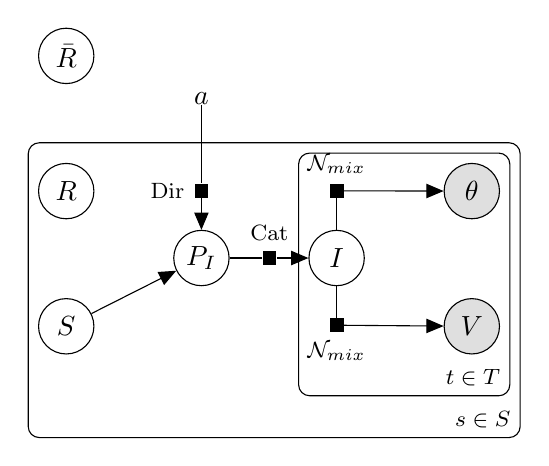
\begin{tikzpicture}
        % NODES
        \node[latent] (I) {$I$};
        \node[obs, right=of I, yshift=0.85cm] (theta) {$\theta$};
        \node[latent, left=of I] (PI){$P_I$};
        \node[obs, below=of theta] (V) {$V$};
        \node[latent, left=of PI, yshift=0.85cm] (R) {$R$};
        \node[latent, above=of R] (RR) {$\bar{R}$};
        \node[latent, below= of R] (S) {$S$};
        
        % FACTORS
        \factor[above=of I] {theta-f}{$\mathcal{N}_{mix}$}{}{};
        \factor[below=of I]{v-f}{below:$\mathcal{N}_{mix}$}{}{};
        \factor[left=of I]{I-f}{Cat}{}{};
        \factor[above=of PI]{PI-f}{left:Dir}{}{};

        \node[const, above=of PI-f] (a) {$a$};
        
        \factoredge {I} {theta-f} {theta};
        \factoredge {I} {v-f} {V};
        \factoredge{PI}{I-f}{I};
        \factoredge{a}{PI-f}{PI};

        \edge{S}{PI};

        \plate {ship}{(I)(theta)(V)}{$t \in T$};
        \plate {}{(I)(theta)(V)(R)(S)(ship)}{$s \in S$};
        
        
    \end{tikzpicture}
\end{figure}

\chapter{Neccessary Theoretical Background}

\section{Useful Results From Probability Theory}


 
\subsection{Conditional Probabilities}
The conditional probability $p(A | B)$ is the probability of $A$ occurring, given that we know $B$ has occured. 
\begin{equation}
    p(A | B) = \frac{p(A, B)}{p(B)}
\end{equation}



\section{Bayesian Statistics}

\section{Stochastic Modelling}

\section{Probabilistic Graphical Models}

\section{Belief Propagation}

\section{Markov Chains}


\chapter{Survey of Training Methods}

\section{Markov-Chain-Monte-Carlo}

\section{Expectation Maximization}

\section{Variational Bayes}

\section{A Note on Probabilistic Programming}


\chapter{Implementation and Results}

This chapter focuses on comparing the performance between \acrshort{mcmc} and \acrshort{vi} methods for performing inference in a \acrshort{pgm}. Each method have their strengths and weaknesses for different types of problems. As a compromise, this chapter will focus on comparing the performance of a fictitious model in order to discuss a concrete example.  

\section{The model}
As the context of this paper is intention inference for autonomous ferries, it seems fit that a similar example is used. A simple intention model is therefore proposed as an example, which relates steering angle to an intention through a mixture model. 

The angle $\theta_t$ is defined to be the angle between the obstacles current course and the predicted course given the obstacles final destination. If the obstacles reported final destination is correct, $D_t=0$, the angle should be closely related to the obstacles intention and can be generated from a Gaussian selected by the intention $I_t$ (i.e. a mixture of Gaussians weighted by the intention probabilities). If the obstacle report an incorrect destination, $D=1$, the angle $\theta_t$ is independent of intention.

Whether or not the final destination is valid is modelled using a Bernoulli variable $D_t$ which takes the value $1$ if the destinations is \textbf{invalid}. A Beta distribution is used to model the prior probability of $D=1$, i.e. the destination being invalid.  

\begin{equation}
    p_D \sim \text{Beta}, \quad p_D \in (0, 1)
\end{equation}
\begin{equation}
    D_t \sim \text{Bernoulli}(p_D), \quad D_t \in \{0, 1\}
\end{equation}

The intention in a situation $I_t$ is modelled by a Categorical discrete variable where the possible realizations are shown in \cref{tbl:intentions}. The intention probabilities $\boldsymbol{\alpha}$ are distributed according to a Dirichlet distribution.

\begin{equation}
    \boldsymbol{\alpha} \sim \text{Dirichlet}, \quad \boldsymbol{\alpha} \in \{\alpha_0, \alpha_1, \alpha_2 \in (0, 1) \; | \; \sum_i \alpha_i = 1 \}
\end{equation}
\begin{equation}
    I_t \sim \text{Categorical}(\boldsymbol{\alpha}), \quad I_t \in \{0, 1, 2\}
\end{equation}

\begin{table}[h]
\centering
\begin{tabular}{|l|l|}
\hline
$I_t=0$ & The obstacle intends to keep its current course \\ \hline
$I_t=1$ & The obstacle intends a starboard turn           \\ \hline
$I_t=2$ & The obstacle intends a portside turn            \\ \hline
\end{tabular}
\caption{Possible realizations of the intention $I_t$}
\label{tbl:intentions}
\end{table}


The mixture components for $\theta_t$ when $D_t=0$ are Gaussian Distributions with unknown mean and variance. The mean and variance for component $I=i$ is 
\begin{align}
    \mu_{i} &\sim \text{Gaussian} & \sigma_i &\sim \text{Inv-Gamma}
\end{align}
When $D=0$ and $I_t=i$, the angle is distributed according to
\begin{equation}\label{eq:theta_intention_mixture}
    \theta_t^{(I=i)} \sim \mathcal{N}_{I=i}(\mu_i, \sigma_i^2), \quad \theta_t^{I=i} \in \mathcal{R}
\end{equation}

One issue with using Guassian for angle information is that the Gaussian Distribution has support on $\mathcal{R}$, while the angles $\theta$ should ideally only have support on $(-\pi, \pi)$. In practice, this may not be a big issue as long as the probability mass is mostly kept within $(-\pi, \pi)$. Another solution could be to use a nonlinear transformation to clamp $\mathcal{R}$ to $(-\pi, \pi)$.

\cref{fig:intention_angle} shows the likelihood for different angles for the different intentions with fixed mean and variance. 

When the obstacles target destination is invalid, $D=1$, the angle $\theta$ is distributed according to a Uniform distribution over the range $(-\pi, \pi)$ to model how the angle contains no information about the obstacle in such a case. 

\begin{equation}
    \theta_t^{(D=1)} \sim \text{Uniform}(-\pi, \pi)
\end{equation}


The data generating process for $\theta_t$ then becomes:

\begin{enumerate}
    \item Draw priors $p_D$, $\boldsymbol{\alpha}$ 
    \item Draw priors $\mu_i$ and $\sigma_i$ for all intentions 
    \item Draw $D_t$ and $I_t$ conditional on $p_D$ and $\boldsymbol{\alpha}$
    \item If $D_t=1$, draw $\theta_t$ from Uniform distribution. If not, draw $\theta_t$ from $\mathcal{N}_{I=i}$ conditional on $\mu_i$ and $\sigma_i$.
\end{enumerate}


\begin{figure}
    \centering
    \includegraphics[width=0.8\textwidth]{figures/intention_angle.png}
    \caption{Normalized likelihood of different angles under different intention hypotheses. This is a polar plot where the angle represent $\theta_t^{(I=i)}$, the radius represent the probability. This is generated from \cref{eq:theta_intention_mixture} with $\mu_0=0$, $\mu_1 = \frac{\pi}{2}$, $\mu_2=-\frac{\pi}{2}$ and $\sigma_i=\frac{\pi}{8}$}
    \label{fig:intention_angle}
\end{figure}


\section{Dataset \& Benchmark}
\section{Markov Chain Monte Carlo}
\section{Variational Inference}
\chapter{Discussion}

All of the methods described in this thesis so far have their strong advantages and disadvantages. 

\section{When all variables are discrete}
In the case of \acrshort{pgm}'s with only discrete variables, exact inference methods are often applicable. The challenges of Bayesian inference in such networks usually boils down to computational complexity when the number of variables increases and in which order the computations should be made. Exact methods such as \acrshort{bp} are in most cases the most appropriate choice, though some structures (in the case of loops) cannot guarantee an optimal solution. 

\section{When some variables are continuous}
When some variables are continuous, the problem usually gets a bit more complicated. If all parent-child can be expressed using conjugate-priors, such as the case of Gaussian Belief Networks, exact methods can still be used. However, requiring the use of only conjugate-priors may in many cases be too restrictive as it limits the ability to express intuitive understanding of the data-generating process. 

The most straight-forward approach will be to use \acrshort{mcmc} methods, due to their inherent simplicity. These methods allow sampling from arbitrarily complex models as long as the target probability can be evaluated. It can in most cases provide asymptotic guarantees that the samples is from the true posterior distribution, though only given a very large amount of samples. How many samples that are considered "enough" is difficult to say, and it usually require manual interpretations of the results in order to verify convergence. Using \acrshort{mcmc} in autonomous systems may therefore be challenging unless the model is sufficiently simple, in which case other methods may still be preferable. Due to the random nature of sampling methods, \acrshort{mcmc} is likely a poor choice for problems where deterministic behaviour is valued. 

In the examples above, \acrshort{mcmc} used more than $8$ minutes sampling, compared to less $25$ seconds for \acrshort{vi} on the same model. Optimizations can most likely be made to significantly speed up both \acrshort{mcmc} and \acrshort{vi}, though the \acrshort{mcmc} will be limited to the large number of required samples needed for accurate results. 



Though it requires more work, \acrshort{vi} will in many cases be a better option. By posing the problem as a optimization problem rather than relying on sampling, variational inference can give deterministic behaviour as well as drastically speed up inference when compared to \acrshort{mcmc}. In the examples above, it took less than $25$ seconds to optimize with a fixed number of iterations, and by inspecting the ELBO it becomes obvious that the training time can be further reduced by early stopping when the learning rate start to diminish. 
However, \acrshort{vi} requires manual selection of a good surrogate density, and the choice of a bad surrogate may lead to poor results due to invalid assumptions. \acrshort{vi} does therefore by itself not provide any guarantees on the correctness of the results as it will always be limited by the assumptions and approximations used by the surrogate density. In the case of complex posterior densities, it may also be challenging to find a proper functional representation of the distribution. As already seen in \cref{fig:example_mcmc_posterior}, the true posterior found by \acrshort{mcmc} does not resemble any known probability distribution. 

A lot of research is currently focusing on how to apply \acrshort{vi} on more complicated models without the need of error-prone calculations or strict assumption. Methods such as variational message passing allows for more complicated surrogate densities in order to retain the interaction between variables in the model \cite{winnbishop}. 

In practice, both methods are likely needed. \acrshort{mcmc} methods can be used to "blindly" sample from the true posterior in order to aid the selection of a proper surrogate density. \acrshort{vi} can then be used to approximate the true posterior without loosing information to invalid assumptions. 

\section{}


\input{chapters/6-conclusion.tex}

\chapter*{\bibname}
\printbibliography[heading=none]

\appendix
\chapter{Result Table from statistical testing}
\begin{table}
    \begin{subtable}{\textwidth}
        \makebox[\textwidth][c]{
            \begin{tabular}{lllrrrrr}
                \toprule
                        &                & Time [Minutes]        & 5       & 10      & 15       & 20       & 25       \\
                Summary & Method         & Training Source       &         &         &          &          &          \\
                \midrule
                Mean    & CVM            & COG/SOG from AIS      & 183     & 405     & 652      & 802      & 1151     \\
                        & Direct GP      & \bf Position          & \bf 532 & \bf 685 & \bf 915  & \bf 1274 & \bf 1636 \\
                        & GP-EKF         & COG/SOG from AIS      & 350     & 704     & 1153     & 1704     & 1975     \\
                        &                & \bf Finite Difference & \bf 359 & \bf 681 & \bf 1060 & \bf 1522 & \bf 1909 \\
                        & GP-EKF w/ PDAF & COG/SOG from AIS      & 341     & 679     & 1030     & 1434     & 1638     \\
                        &                & \bf Finite Difference & \bf 341 & \bf 638 & \bf 972  & \bf 1396 & \bf 1753 \\
                        & GP-EKF w/ SL   & COG/SOG from AIS      & 341     & 680     & 1105     & 1634     & 1879     \\
                        &                & \bf Finite Difference & \bf 353 & \bf 667 & \bf 1029 & \bf 1476 & \bf 1778 \\
                \midrule
                Median  & CVM            & COG/SOG from AIS      & 96      & 210     & 358      & 464      & 721      \\
                        & Direct GP      & \bf Position          & \bf 312 & \bf 503 & \bf 649  & \bf 992  & \bf 1266 \\
                        & GP-EKF         & COG/SOG from AIS      & 292     & 577     & 994      & 1598     & 1876     \\
                        &                & \bf Finite Difference & \bf 297 & \bf 538 & \bf 835  & \bf 1285 & \bf 1474 \\
                        & GP-EKF w/ PDAF & COG/SOG from AIS      & 279     & 550     & 807      & 1141     & 1263     \\
                        &                & \bf Finite Difference & \bf 289 & \bf 511 & \bf 752  & \bf 1115 & \bf 1563 \\
                        & GP-EKF w/ SL   & COG/SOG from AIS      & 285     & 545     & 939      & 1530     & 1869     \\
                        &                & \bf Finite Difference & \bf 287 & \bf 518 & \bf 813  & \bf 1246 & \bf 1346 \\
                \bottomrule
            \end{tabular}
        }
        \caption{Trajectory errors in meters}
        \label{table:stats_straight_traj_err}
        \vspace*{0.5cm}
    \end{subtable}
    \begin{subtable}{\textwidth}
        \makebox[\textwidth][c]{
            \begin{tabular}{lllrrrrr}
                \toprule
                        &                & Time [Minutes]        & 5       & 10      & 15      & 20      & 25      \\
                Summary & Method         & Training Source       &         &         &         &         &         \\
                \midrule
                Mean    & CVM            & COG/SOG from AIS      & 52      & 150     & 284     & 344     & 582     \\
                        & Direct GP      & \bf Position          & \bf 258 & \bf 239 & \bf 344 & \bf 473 & \bf 701 \\
                        & GP-EKF         & COG/SOG from AIS      & 78      & 140     & 202     & 249     & 286     \\
                        &                & \bf Finite Difference & \bf 80  & \bf 148 & \bf 224 & \bf 265 & \bf 332 \\
                        & GP-EKF w/ PDAF & COG/SOG from AIS      & 100     & 198     & 311     & 354     & 389     \\
                        &                & \bf Finite Difference & \bf 81  & \bf 149 & \bf 234 & \bf 279 & \bf 404 \\
                        & GP-EKF w/ SL   & COG/SOG from AIS      & 76      & 132     & 188     & 231     & 266     \\
                        &                & \bf Finite Difference & \bf 79  & \bf 140 & \bf 207 & \bf 243 & \bf 306 \\
                \midrule
                Median  & CVM            & COG/SOG from AIS      & 28      & 70      & 136     & 223     & 411     \\
                        & Direct GP      & \bf Position          & \bf 76  & \bf 120 & \bf 197 & \bf 258 & \bf 419 \\
                        & GP-EKF         & COG/SOG from AIS      & 58      & 99      & 142     & 180     & 233     \\
                        &                & \bf Finite Difference & \bf 65  & \bf 105 & \bf 157 & \bf 167 & \bf 223 \\
                        & GP-EKF w/ PDAF & COG/SOG from AIS      & 60      & 104     & 149     & 184     & 240     \\
                        &                & \bf Finite Difference & \bf 66  & \bf 104 & \bf 147 & \bf 179 & \bf 205 \\
                        & GP-EKF w/ SL   & COG/SOG from AIS      & 55      & 94      & 132     & 159     & 192     \\
                        &                & \bf Finite Difference & \bf 63  & \bf 101 & \bf 139 & \bf 155 & \bf 199 \\
                \bottomrule
            \end{tabular}


        }
        \caption{Path error in meters}
        \label{table:stats_straight_path_err}
    \end{subtable}
    \caption{Error summary for $350$ straight-line trajectories. Mean and median summary statistics are calculated for the trajectory and path error at fixed timestamps. Linear interpolation is used between samples. Errors for short trajectories are not extrapolated, and therefore not included in the $20$ and $25$ minute bins.}
    \label{table:stats_straight_line_error}
\end{table}

\begin{table}
    \begin{subtable}{\textwidth}
        \makebox[\textwidth][c]{
            \begin{tabular}{lllrrrrr}
                \toprule
                        &                & Time [Minutes]         & 5       & 10      & 15      & 20       & 25       \\
                Summary & Method         & Training Source        &         &         &         &          &          \\
                \midrule
                Mean    & CVM            & COG/SOG from AIS       & 440     & 1071    & 1898    & 2425     & 3313     \\
                        & Direct GP      & \bf Position           & \bf 366 & \bf 522 & \bf 771 & \bf 993  & \bf 1298 \\
                        & GP-EKF         & COG/SOG from AIS       & 352     & 674     & 950     & 1327     & 1856     \\
                        &                & \bf Finite Difference  & \bf 329 & \bf 575 & \bf 823 & \bf 1081 & \bf 1388 \\
                        & GP-EKF w/ PDAF & COG/SOG from AIS       & 478     & 904     & 1255    & 1473     & 1824     \\
                        &                & \bf Finite Difference  & \bf 371 & \bf 610 & \bf 835 & \bf 1056 & \bf 1220 \\
                        & GP-EKF w/ SL   & COG/SOG from AIS       & 340     & 636     & 874     & 1194     & 1592     \\
                        &                & \bf Finite Difference  & \bf 324 & \bf 555 & \bf 795 & \bf 1030 & \bf 1312 \\
                \hline
                Median  & CVM            & COG/SOG from AIS       & 167     & 452     & 1009    & 1561     & 2359     \\
                        & Direct GP      & \bf Position           & \bf 229 & \bf 364 & \bf 550 & \bf 705  & \bf 942  \\
                        & GP-EKF         & COG/SOG from AIS       & 257     & 483     & 724     & 1078     & 1505     \\
                        &                & \bf Finite Difference  & \bf 255 & \bf 463 & \bf 635 & \bf 844  & \bf 1120 \\
                        & GP-EKF w/ PDAF & COG/SOG from AIS       & 368     & 654     & 923     & 1128     & 1327     \\
                        &                & \bf Finite Difference  & \bf 315 & \bf 493 & \bf 651 & \bf 704  & \bf 854  \\
                        & GP-EKF w/ SL   & COG/SOG from AIS       & 251     & 452     & 646     & 989      & 1357     \\
                        &                & \bf  Finite Difference & \bf 256 & \bf 434 & \bf 626 & \bf 789  & \bf 1113 \\
                \bottomrule
            \end{tabular}
        }
        \caption{Trajectory Error in meters}
        \label{table:stats_curved_traj_err}
        \vspace*{0.5cm}
    \end{subtable}
    \begin{subtable}{\textwidth}
        \makebox[\textwidth][c]{
            \begin{tabular}{lllrrrrr}
                \toprule
                        &                & Time [Minutes]         & 5        & 10       & 15      & 20      & 25       \\
                Summary & Method         & Training Source        &          &          &         &         &          \\
                \midrule
                Mean    & CVM            & COG/SOG from AIS       & 204      & 574      & 1072    & 1518    & 2045     \\
                        & Direct GP      & \bf Position           & \bf 175  & \bf 231  & \bf 403 & \bf 596 & \bf 827  \\
                        & GP-EKF         & COG/SOG from AIS       & 143      & 269      & 356     & 484     & 687      \\
                        &                & \bf Finite Difference  & \bf 160  & \bf 291  & \bf 412 & \bf 466 & \bf 509  \\
                        & GP-EKF w/ PDAF & COG/SOG from AIS       & 177      & 355      & 587     & 775     & 1218     \\
                        &                & \bf Finite Difference  & \bf 155  & \bf 277  & \bf 413 & \bf 515 & \bf  655 \\
                        & GP-EKF w/ SL   & COG/SOG from AIS       & 137      & 240      & 300     & 392     & 522      \\
                        &                & \bf Finite Difference  & \bf 151  & \bf 265  & \bf 375 & \bf 437 & \bf 523  \\
                \hline
                Median  & CVM            & COG/SOG from AIS       & 54       & 265      & 715     & 1138    & 1863     \\
                        & Direct GP      & \bf Position           & \bf 81   & \bf 140  & \bf 234 & \bf 336 & \bf 447  \\
                        & GP-EKF         & COG/SOG from AIS       & 99       & 152      & 216     & 295     & 408      \\
                        &                & \bf Finite Difference  & \bf 106  & \bf 180  & \bf 323 & \bf 336 & \bf  377 \\
                        & GP-EKF w/ PDAF & COG/SOG from AIS       & 97       & 157      & 290     & 401     & 908      \\
                        &                & \bf  Finite Difference & \bf  101 & \bf  182 & \bf 304 & \bf 371 & \bf 402  \\
                        & GP-EKF w/ SL   & COG/SOG from AIS       & 92       & 133      & 195     & 227     & 302      \\
                        &                & \bf  Finite Difference & \bf 101  & \bf 173  & \bf 290 & \bf 309 & \bf 395  \\
                \bottomrule
            \end{tabular}
        }
        \caption{Path error in meters}
        \label{table:stats_curved_path_err}
    \end{subtable}
    \caption{Error summary for $350$ curved trajectories. Mean and median summary statistics are calculated for the trajectory and path error at fixed timestamps. Linear interpolation is used between samples. Errors for short trajectories are not extrapolated, and therefore not included in the $20$ and $25$ minute bins.}
    \label{table:stats_curved_error}
\end{table}

\end{document}
